%%
%% This is file `yanputhesis-sample.tex',
%% generated with the docstrip utility.
%%
%% The original source files were:
%%
%% yanputhesis.dtx  (with options: `sample')
%% Copyright (C) 2022 by Shangkun Shen
%% 
%% It may be distributed and/or modified under the conditions of the LaTeX
%% Project Public License, either version 1.3b of this license or (at your
%% option) any later version. The latest version of this license is in
%%     https://www.latex-project.org/lppl.txt
%% and version 1.3b or later is part of all distributions of LaTeX version
%% 2005/12/01 or later.
%%=============================================================================%
%% 设置论文格式(学位、盲评、Adobe 字体)
%%-----------------------------------------------------------------------------%
%% 博士、正常版本、不使用 Adobe 字体
%% \documentclass[lang=chs, degree=phd, blindreview=false, adobe=false]{yanputhesis}
%% 博士、盲评版本、不使用 Adobe 字体
%% \documentclass[lang=chs, degree=phd, blindreview=true, adobe=false]{yanputhesis}
%% 博士、正常版本、强制使用 Windows 系统字体
%%\documentclass[lang=chs, degree=phd, blindreview=false, winfonts=true]{yanputhesis}
%% 硕士、正常版本、不使用 Adobe 字体
\documentclass[lang=chs, degree=master, blindreview=false, adobe=false]{yanputhesis}
%% 硕士、盲评版本、不使用 Adobe 字体
%% \documentclass[lang=chs, degree=master, blindreview=true, adobe=false]{yanputhesis}
%%=============================================================================%
%% 导言区:请自行添加额外宏包
%%-----------------------------------------------------------------------------%
\usepackage{blindtext}                                      % 生成无意义文本
\usepackage{metalogo}                                       % 软件标志
\usepackage[binary-units=true]{siunitx}                     % 物理量单位
\usepackage{amsmath}                                        % 基础数学库
%%=============================================================================%
%% 参考文献(也可以是独立文件)
%%-----------------------------------------------------------------------------%
\begin{filecontents}{reference.bib}
@software{NWPUThesisLaTeXTemplate,
  title     = {Yet Another {{\LaTeX}} Template for NPU Thesis},
  author    = {Shangkun Shen and Zhihe Wang and Jiduo Zhang and Weijia Zhang},
  month     = {11},
  year      = {2019},
  publisher = {Zenodo},
  journal   = {GitHub repository},
  doi       = {10.5281/zenodo.4159248},
  url       = {https://doi.org/10.5281/zenodo.4159248}
}

@book{knuth1986the,
  title     = {The {{\TeX}}book},
  author    = {Knuth, Donald E},
  publisher = {Addison-Wesley},
  year      = {1986}
}

@book{lamport1989latex,
  title     = {{{\LaTeX}}: a document preparation system},
  author    = {Lamport, Leslie},
  publisher = {Addison-Wesley Professional},
  year      = {1989}
}

@article{szegedy2015going,
  title   = {Going deeper with convolutions},
  author  = {Szegedy, Christian and Liu, Wei and Jia, Yangqing and
             Sermanet, Pierre and Reed, Scott E and Anguelov, Dragomir and
             Erhan, Dumitru and Vanhoucke, Vincent and Rabinovich, Andrew},
  journal = {Computer Vision and Pattern Recognition},
  pages   = {1--9},
  year    = {2015}
}

@software{MathSymbolsinLaTeXbypolossk,
  title     = {Math Symbols in {{\LaTeX}}},
  author    = {Shangkun Shen},
  year      = {2017},
  month     = {10},
  publisher = {Zenodo},
  journal   = {GitHub repository},
  doi       = {10.5281/zenodo.4120375},
  url       = {https://doi.org/10.5281/zenodo.4120375}
}

@article{chen2014maiyuan,
  title   = {脉源三支 强强融合——西北工业大学},
  author  = {{陈家忠}},
  journal = {电子技术与软件工程},
  number  = {9},
  pages   = {15--16},
  year    = {2014}
}

@article{shen2021peridynamic,
  title     = {Peridynamic modeling with energy-based surface correction for
               fracture simulation of random porous materials},
  journal   = {Theoretical and Applied Fracture Mechanics},
  volume    = {114},
  pages     = {102987},
  year      = {2021},
  issn      = {0167-8442},
  author    = {Shangkun Shen and Zihao Yang and Fei Han and Junzhi Cui and
               Jieqiong Zhang},
  publisher = {Elsevier}
}

@inproceedings{chen2018autonomous,
  title        = {Autonomous vehicle testing and validation platform: Integrated
                  simulation system with hardware in the loop},
  author       = {Chen, Yu and Chen, Shitao and Zhang, Tangyike and
                  Zhang, Songyi and Zheng, Nanning},
  booktitle    = {2018 IEEE Intelligent Vehicles Symposium (IV)},
  pages        = {949--956},
  year         = {2018},
  organization = {IEEE}
}
\end{filecontents}
%%=============================================================================%
%% 基本信息录入
%%-----------------------------------------------------------------------------%
\title{半监督遥感影像 \\ 变化检测算法研究}{          % 中英文标题
   Research on semi-supervised \\ remote Sensing image change detection algorithm
}                                                           % 请自行断行
\author{\blindreview{温冬成}}{\blindreview{Dongcheng Wen}}  % 姓名(添加盲评标记)
\date{2025年4月}{April 2025}                                  % 答辩日期
\school{计算机学院}{School of Computer science}% 学院
\major{计算机技术}{Computer technology}                     % 专业 博士请添加 Ph
\advisor{\blindreview{冉令燕}}{\blindreview{Lingyan Ran}}      % 导师(添加盲评标记)
\studentnumber{2022262929}                                  % 学号

%%=============================================================================%
%% 文档开始
%%-----------------------------------------------------------------------------%
\begin{document}
%%-----------------------------------------------------------------------------%
%% 总前言,包含封皮页、中英文标题、中英文摘要、目录
%%-----------------------------------------------------------------------------%
\frontmatter                                                % 前言部分
\maketitle                                                  % 封皮页及标题页
%%-----------------------------------------------------------------------------%
\makeCommitteePage{                                         % 学位论文评阅人
    \reviewers{\fullBlindReview{5}}                         % 和答辩委员会名单
    \committee{2023 年 x 月 y 日}{
        \defenseChair{赵钱孙}{教授}{西北工业大学}
        \committeeMember{周吴郑}{教授}{西北工业大学}
        \committeeMember{冯陈褚}{教授}{西北工业大学}
        \committeeMember{蒋沈韩}{教授}{西北工业大学}
        \committeeMember{朱秦尤}{教授}{西北工业大学}
        \committeeMember{何吕施}{教授}{西北工业大学}
        \committeeMember{孔曹严}{教授}{西北工业大学}
        \defenseSecretary{金魏陶}{教授}{西北工业大学}
    }
}
%%-----------------------------------------------------------------------------%
\begin{abstract}                                            % 中文摘要开始
    这是在西北工业大学本科毕业设计、硕博研究生毕业论文格式的要求下的一份 LaTeX
    文档类模板。使用者无需额外修改格式控制细节,直接在所发布的样例基础上,修改章
    节标题,撰写内容,即可完成毕业设计论文任务。            %
    \begin{keywords}                                        % 中文关键词开始
        学位论文 \sep 模板 \sep \LaTeX                      %
    \end{keywords}                                          % 中文关键词结束
\end{abstract}                                              % 中文摘要结束
%%-----------------------------------------------------------------------------%
\begin{engabstract}                                         % 英文摘要开始
    \noindent \blindtext                                    %
    \begin{engkeywords}                                     % 英文关键词开始
        thesis \ensep template \ensep \LaTeX                %
    \end{engkeywords}                                       % 英文关键词结束
\end{engabstract}                                           % 英文摘要结束
%%-----------------------------------------------------------------------------%
\tableofcontents                                            % 目录
\listoffigures                                              % 图目录(学校未做要求)
\listoftables                                               % 表目录(学校未做要求)
\printnomenclature                                          % 符号表(学校未做要求)
%%-----------------------------------------------------------------------------%
\mainmatter
\sDefault
\chapter{绪论}
\chaptermark{绪论}
\section{研究背景与意义}
随着科技水平的不断进步,人类的生产、生活对于自然界和人类世界都以更快的速度发挥着更重要的影响力,在以往可能经过数十年乃至几个世纪间的自然演变过程才造成的地球地形地貌变化,例如河流改道、填海填湖,在如今或许被缩短至数年甚至数月,观测和把握这种变化对我们分析和指导生产活动是一件非常重要的事情。目前相关的对地观测技术也得到了飞速的发展,人们借助于高空无人机和遥感卫星的对地传感器能够轻松完成对地球表面的信息采集,并实时返回遥感影像数据,这已经逐渐成为了人们了解和观测地球的主要方式。并且现代遥感成像技术的成熟也使得采集到的遥感图像具有较高的空间分辨率,从而为人们动态检测地表变化提供了可能性和便利性。

所谓的遥感影像变化检测(Remote sensing change detection, RSCD),本质上是一个二分类的问题,就是在卫星对于同一区域在不同时间拍摄的双时相图像对中,识别出感兴趣的目标变化区域,比如建筑物、水域、植被和道路。该技术在许多军事领域以及民用应用中发挥着重要作用,例如,城市建设规划、森林环境保护、农村土地管理、自然灾害评估等民用领域和军事监视、导弹命中分析等军事领域。在计算机技术的广泛应用之前,人类主要依靠人工目视法来进行这种变化检测并手动标注变化区域和类型,这种方法虽然可靠,但是依赖于专业研究人员的检测经验,并且在面对海量任务时,这种方法的可行性和经济性就受到了极大的挑战。伴随计算机科学的进步和机器学习的兴起,自动变化检测开始走入了人们的视线,早期广泛采用的基于传统机器学习算法的变化检测方法,其能够处理的遥感图像分辨率相对较低,主要包括:(1)基于图像差分、图像回归、图像比例、变化向量分析(CVA)等代数方法;(2)基于变换的方法,如主成分分析(PCA)、多元变化检测(MAD)、Gramm-Schmidt变化分析(GS)等,通过将高维特征投影到低维特征空间中,使特征分量去相关,从而突出重要的变化信息表示。(3)基于分类方法。例如,后分类比较方法。该方法首先对前后时间图像进行独立分类,然后逐像素比较两幅图像的分类结果,既可以回答“哪里发生了变化”的问题,也可以回答专家感兴趣的另一个问题“发生了什么变化”,但缺点也很明显,即高度依赖高精度高配准的分类结果,实施起来难度极大。

\begin{figure}[htb]
	\centering
	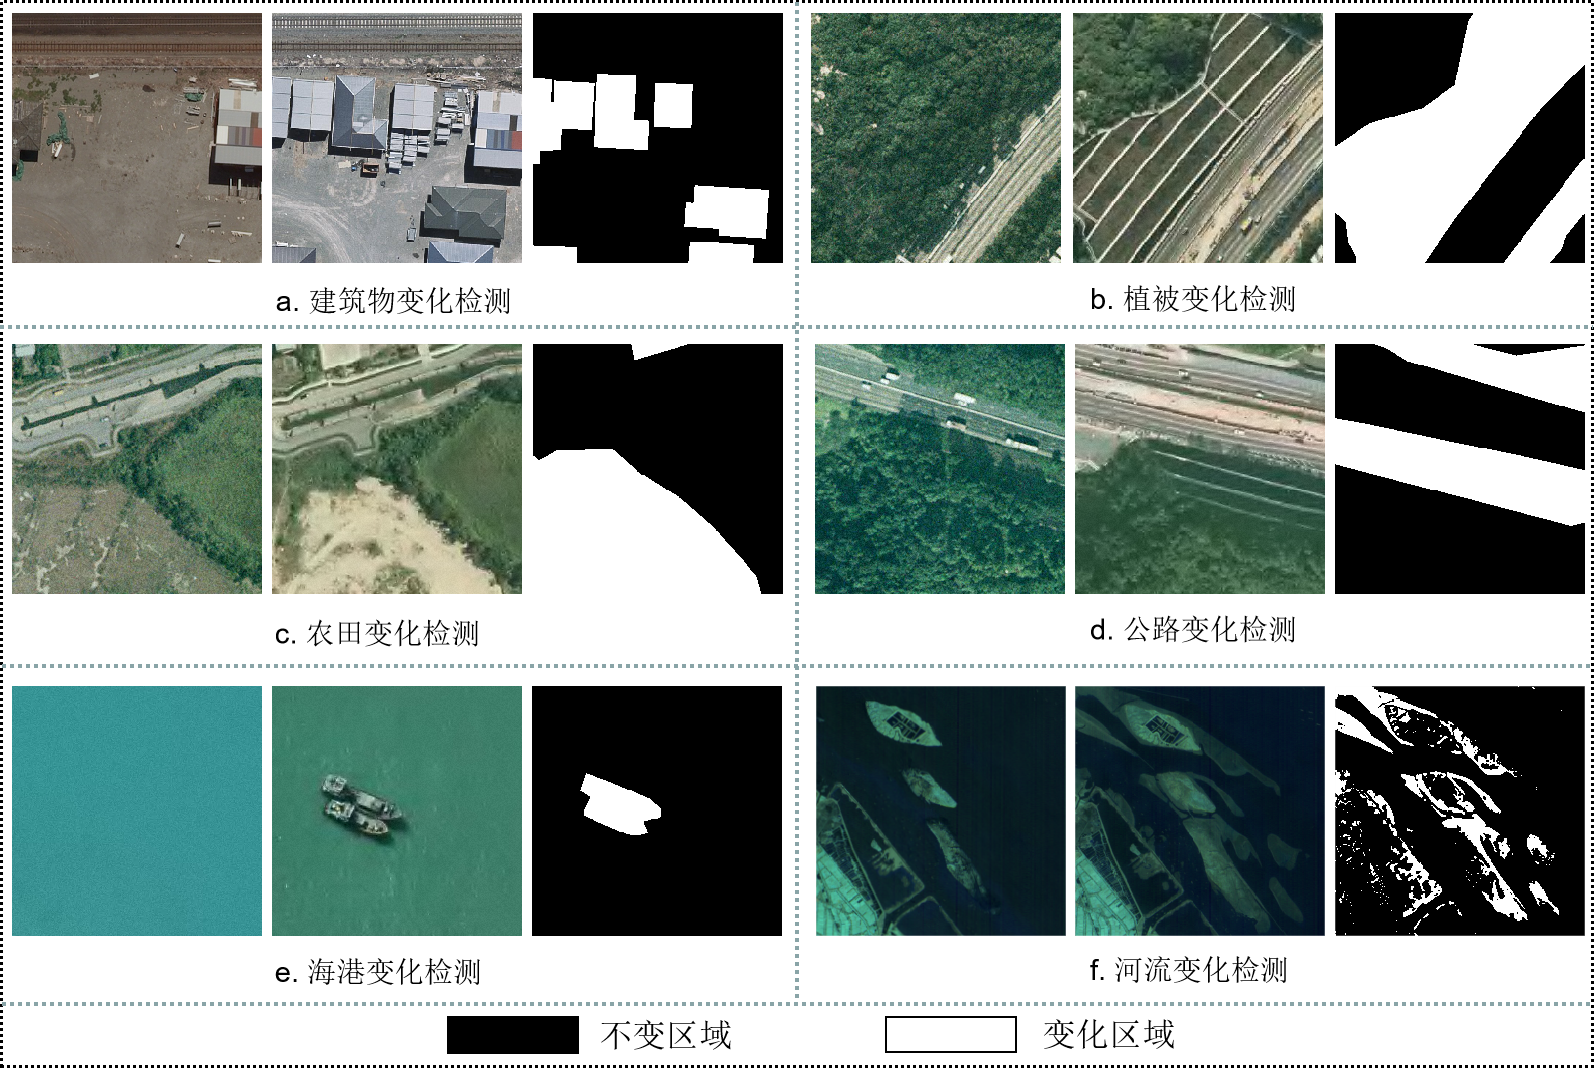
\includegraphics[scale=0.6]{images/fig1.png}
	\caption{
		变化检测在各种领域的应用
	}
	\label{fig:background}
\end{figure}

目前,深度学习算法已经被广泛应用到各种计算机视觉任务,比如图像分类、目标检测、深度估计,以及语义分割、实例分割等与变化检测相似的密集预测任务,并且表现出了远超传统方法的优异性能。然而,基于卷积神经网络(Convolutional Neural Network, CNN)或者Transformer网络的全监督的深度学习变化检测算法都及其依赖于大量的人工标注,当有标注的训练样本减少时,模型的识别能力急剧下降。而且,变化检测任务的数据标注非常复杂,需要高精度几何图像配准和像素级精细标注,耗时耗力。这一点从目前可以获取到的公开数据集的数据规模对比就可以看出来,通常图像分类、目标检测的数据集能够达到数十万张,而变化检测的数据集规模仅在几百至几万张。为了应对这些挑战,研究人员研究了一系列方法,如自监督学习(Self-supervised learning, SSL)、无监督变化检测(Unsupervised Change Detection, USCD)、弱监督变化检测(Weakly Supervised Change Detection, WSCD)和样本生成策略(sample generation strategies)。虽然弱监督变化检测具有一定的成本效益,但它依赖于不完整或不准确的标签,这可能会引入错误信号和不可预测的噪声数据。另一方面,无监督变化检测完全不使用标注数据,而是利用数据中存在的固有联系作为监督指导,这导致它在处理分类或检测等特定任务时,由于缺乏正确的语义信息而面临挑战。样本生成策略,包括数据增强[23]、生成式对抗网络和扩散模型,经常需要模拟或合成额外的数据样本。然而,当处理有限的可用样本时,由于生成的数据多样性不足,这些方法可能会遇到约束,从而降低模型的泛化能力。半监督变化检测有效弥补了这些方法的不足,一方面它能够从有限的标注数据中学习到正确的语义信息,另一方面还能够从大量的易获得的无标注数据分布中学习到更为多样的变化特征表示,因此,半监督变化检测成为了一种更有前景的解决方案。

在此研究背景之下,本文着力研究了半监督变化检测算法,针对模型为无标注样本生成的伪标签可能包含错误标签从而引入额外噪声这一问题,我们从提高无标注样本的伪标签的可靠性入手进行了一系列的研究,分别从无标注样本增强、模型参数更新、伪标签生成模型、伪标签生成策略等方面进行了改进,有效地提升了伪标签的质量,从而提高了半监督变化检测算法的性能。

\section{国内外研究现状及趋势}
此前国内外学者已经在半监督变化检测算法领域进行了大量的研究,本小节将介绍与本文最相关的几个方向的研究现状,包括半监督学习,全监督遥感影像变化检测,以及半监督遥感影像变化检测的基本任务与方法和研究发展历程。
\subsubsection{半监督学习算法}
在实际应用场景中,无标签的数据易于获取,而有标签的数据收集起来通常很困难,标注过程也是一项极度劳动密集的工作。在这种情况下,半监督学习(Semi-Supervised Learning, SSL)是一种克服样本标注困难问题的可行方法,近年来也已经成为深度学习领域一个热门的研究方向,其旨在仅利用一小部分标记数据进行监督训练,学习到正确的语音信息,同时利用大量的无标注训练样本进行无监督训练,以提高模型的泛化性,减少过拟合现象。SSL主要包含三种策略:一致正则化(Consistent Regularization, CR)、自训练(Self Training)、生成模型以及一些包括其中多种思想的整体方法。

一致性正则化方法基于扰动一致性的概念,所谓的扰动一致性即:如果对一个未标记的数据应用实际的扰动,则预测不应发生显著变化,因为在聚类假设下,具有不同标签的数据点在低密度区域是互相分离的。这种方法首先对输入数据施加不同程度的扰动,将模型在这些输入数据上的输出之间的一致性作为训练约束。目前的三个主流的一致性正则化训练框架包括:Π-模型[35],时间集成模型[35]和平均教师(Mean-Teacher, MT)模型[32]。这几种框架都是以双分支网络作为基础架构,其中Π-模型的双分支网络之间是共享参数权重的;时间集成模型合并时间序列中的所有输出,每个图像的伪标签是先前生成结果的EMA;MT模型在模型参数水平上进行平滑操作。该模型在随后的各个领域的半监督研究中得到了应用,例如Active-Teacher用于半监督对象检测[36],[33],[37]-[39]用于半监督一般语义分割,[40]用于图像分类,[41][42]用于半监督医学图像分割。在摄动设计领域也进行了探索,[43]和[25]分别检测了CR的图像级摄动和特征级摄动。
\subsubsection{遥感影像变化检测}
emmm
\subsubsection{半监督遥感影像变化检测}
emmm
\section{本文主要内容及结构安排}
emmm
\chapter{基于深度学习的变化检测网络和半监督学习算法}
\section{深度变化检测网络}
\section{半监督学习算法}
\section{本章小结}
\chapter{基于伪标签评估的自适应半监督变化检测算法}
\section{引言}
\section{基于伪标签评估的自适应半监督变化检测框架}
\subsection{整体框架}
\subsection{伪标签评估指标设计}
\subsection{自适应样本增强机制}
\subsection{自适应师生模型参数更新机制}
\section{实验结果及分析}
\subsection{变化检测数据集介绍}
\subsection{评估指标}
\subsection{实验设置}
\subsection{对比试验}
\subsection{消融实验}
\section{本章小结}
\chapter{基于伪标签评估的自适应半监督变化检测算法}
\section{引言}


\chapter{基于SAM改善伪标签的半监督变化检测算法}
\section{引言}
\section{基于SAM改善伪标签的半监督变化检测框架}
\subsection{整体框架}
\subsection{基于双时分割掩码差分的伪标签生成}
\subsubsection{像素级差分算法}
\subsubsection{实例级差分算法}
\subsection{基于双时特征差分的伪标签生成}
\section{实验结果及分析}
\subsection{实验设置}
\subsection{对比试验}
\subsection{消融实验}
\section{本章小结}

\chapter{基于APE的单模型半监督变化检测算法}
\section{引言}
\section{基于APE的单模型半监督变化检测框架}
\subsection{整体框架}
\subsection{基于查询的自动伪标签生成}
\section{实验结果及分析}
\subsection{实验设置}
\subsection{对比试验}
\subsection{消融实验}
\section{本章小结}


\cleardoublepage
%%=============================================================================%
%% 参考文献以及附录
%%-----------------------------------------------------------------------------%
%% \bibliographystyle{nputhesis}                               % GB/T 7714-2015 格式
\bibliographystyle{nputhesis-noslash}                       % 参考文献改进格式
\bibliography{reference}                                    % 参考文献
\appendix
\chapter{一份说明 顺便测试英文标题 Title}

强烈不推荐英文标题!仅供测试,擅自使用后果自负。

\section{测试附录子标题}

这是一份附录,请放置一些独立的证明、源代码、或其他辅助资料。

\nomenclature{$r$}{圆(或球)的半径}
\nomenclature{$C$}{圆的周长}
\nomenclature{$S$}{圆的面积}

\begin{equation}
    C = 2 \pi r
\end{equation}

\begin{equation}
    S = \pi r^2
\end{equation}

\cleardoublepage

\chapter{另一份说明}

这是另一份附录,请放置一些独立的证明、源代码、或其他辅助资料。

\nomenclature{$S_{\text{sphere}}$}{球的表面积}
\nomenclature{$V_{\text{sphere}}$}{球的体积}

\begin{equation}
    S_{\text{sphere}} = 4 \pi r^2
\end{equation}

\begin{equation}
    V_{\text{sphere}} = \frac43 \pi r^3
\end{equation}

\cleardoublepage
%%=============================================================================%
%% 文档附页部分(致谢、参加科研情况、知识产权与原创性声明)
%%-----------------------------------------------------------------------------%
\backmatter                                                 % 文档附页部分
%%-----------------------------------------------------------------------------%
\begin{acknowledgements}                                    % 致谢开始
    感谢我的老师和我的朋友们……
\end{acknowledgements}                                      % 致谢结束
%%-----------------------------------------------------------------------------%
\begin{accomplishments}                                     % 参加科研情况开始
    [1] ...
\end{accomplishments}                                       % 参加科研情况结束
%%-----------------------------------------------------------------------------%
\makestatement                                              % 知识产权与原创性声明
%%=============================================================================%
%% 文档结束
%%-----------------------------------------------------------------------------%
\end{document}
%%=============================================================================%


%% 
%% This work consists of the file  yanputhesis.dtx
%% and the derived files           yanputhesis.ins,
%%                                 yanputhesis.pdf,
%%                                 yanputhesis.cls.
%% 
%%
%% End of file `yanputhesis-sample.tex'.
